\documentclass[11pt]{article}
% =====================================================================
%  I2S-anti (I2S-A) family --- the three program-feature categories.
%  Companion to i2s_pro_categories.tex. Every cited branch + value is REAL
%  (from bench/dataset.jsonl + the per-branch analysis cards); libpng/3977
%  is verified against local source, the harfbuzz gates from their cards.
%  Compile: pdflatex i2s_anti_categories.tex   (tikz + pgfplots + listings)
% =====================================================================
\usepackage[margin=1in]{geometry}
\usepackage{amsmath,amssymb}
\usepackage{xcolor}
\usepackage{listings}
\usepackage{booktabs}
\usepackage{tikz}
\usepackage{pgfplots}
\pgfplotsset{compat=1.16}
\usetikzlibrary{arrows.meta,positioning}

\definecolor{winc}{RGB}{30,120,60}   % winner (the arm that resolves) green
\definecolor{losc}{RGB}{190,60,60}   % loser  (the I2S arm that blocks) red
\definecolor{codebg}{RGB}{246,246,248}
\definecolor{kw}{RGB}{40,60,150}
\definecolor{cmt}{RGB}{120,120,120}
\definecolor{str}{RGB}{160,60,20}

\lstdefinestyle{c}{
  language=C, basicstyle=\ttfamily\small, backgroundcolor=\color{codebg},
  keywordstyle=\color{kw}\bfseries, commentstyle=\color{cmt}\itshape,
  stringstyle=\color{str}, numbers=none, frame=single, framerule=0pt,
  framesep=6pt, breaklines=true, showstringspaces=false, xleftmargin=4pt,
}

% tool / metric / rule / real-example box
\newcommand{\metricbox}[4]{%
  \par\smallskip\noindent\fbox{\parbox{\dimexpr\linewidth-2\fboxsep-2\fboxrule}{%
  \footnotesize
  \textbf{Tool:}~\texttt{#1}\\[2pt]
  \textbf{Metric:}~#2\\[2pt]
  \textbf{Verify rule (deterministic arbiter):}~\texttt{#3}\\[2pt]
  \textbf{Real example:}~#4}}\par\smallskip}

\title{\textbf{The I2S-anti family: three ways input-to-state copying backfires}}
\author{}
\date{}

\begin{document}
\maketitle
\vspace{-3em}

\paragraph{Backdrop.} \emph{I2S-anti} (I2S-A) collects the roadblocks where
input-to-state copying \emph{hurts}: a non-I2S arm resolves the branch but the
I2S-bearing arm blocks it. It is the \emph{same} operand substitution that powers
I2S-pro, turned against the fuzzer --- \texttt{cmplog} logs a comparison operand
and \texttt{I2SRandReplace} splices it back in, but here the spliced value steers
the corpus \emph{away} from what the branch needs. Every case shares one measured
signature: on the campaign corpus the I2S arm is \emph{depleted} of the byte the
winning arm reaches, so the same \texttt{operand\_enrichment} tool fires with the
sign flipped --- \texttt{signed\_target\_enrich}\,$<-0.3$ (versus $\ge+1.0$ for
I2S-pro). The three categories differ only in \emph{what decoy} the substitution
injects. The backfire shows up against either baseline --- \emph{naive}$\,\succ\,$\emph{cmplog}
or \emph{value\_profile}$\,\succ\,$\emph{vpc} (the same substitution hurting plain
havoc, or hurting on top of the value-profile gradient); we merge both because the
program mechanism is identical. Counts are validated roadblocks ($n$).

\smallskip\noindent\textit{A note on the metric.} \texttt{signed\_target\_enrich}
is a sign-preserving, max-magnitude \emph{per-offset} log$_2$ frequency ratio
(cmplog vs naive at the gate offset, with an $\epsilon{=}10^{-6}$ floor). Its
\emph{sign} is the classifier signal (negative $=$ the I2S arm is depleted of the
target byte); its magnitude saturates when the byte is absent at an offset, so a
value like $-13.6$ just means ``essentially gone,'' not a precise ratio.

% =====================================================================
\section*{1.\ \ A rival operand wins the harvest \hfill {\normalsize\texttt{i2s\_anti\_target\_depletion} ($n=25$)}}
The gate needs a specific byte value, and \emph{naive} havoc lands it by chance ---
but I2S keeps splicing a \emph{different}, abundant operand it harvested from some
\emph{other} comparison in the program into the same position, pinning the cmplog
corpus onto that decoy and starving it of the value the branch wants.

\begin{lstlisting}[style=c]
// libpng  pngrutil.c : png_handle_cHRM()   (cHRM chunk, length 32)
xy.bluex = png_get_fixed_point(buf + 24);  // parse the bluex sub-field
if (xy.bluex == PNG_FIXED_ERROR || ...)    // <-- blocker (libpng/3977)
    png_chunk_benign_error(...);           // taken when bluex is out-of-range
\end{lstlisting}

\noindent The branch is taken when \texttt{bluex} parses to an out-of-range
fixed-point (\texttt{PNG\_FIXED\_ERROR}). \emph{naive}'s random bytes hit that
easily (target byte \texttt{0x00}); but \texttt{cmplog} harvests the ASCII float
exponent \texttt{'e'} (\texttt{0x65}) from \emph{other} numeric comparisons in the
parser (e.g.\ from \texttt{"1.0e0"}, \texttt{"65.535"}) and splices it into the
\texttt{bluex} bytes, producing an in-range value that does \emph{not} trip the
gate --- so the I2S corpus is pinned to the decoy and depleted of the target.

\metricbox{operand\_enrichment}
{\texttt{signed\_target\_enrich} (target byte) and \texttt{decoy\_enrich} (the rival byte), both log$_2$ cmplog/naive ratios}
{skip != no\_gate\_signature AND signed\_target\_enrich < -0.3}
{libpng/3977 (\texttt{cHRM} handler, \texttt{pngrutil.c:1283}) --- the decoy \texttt{'e'} fills 63\% of the cmplog corpus (vs 39\% naive) while the target byte drops to 8.9\% (vs 15.7\% naive): \texttt{signed\_target\_enrich}$=-0.82$, \texttt{decoy\_enrich}$=+0.68$.}

\begin{center}
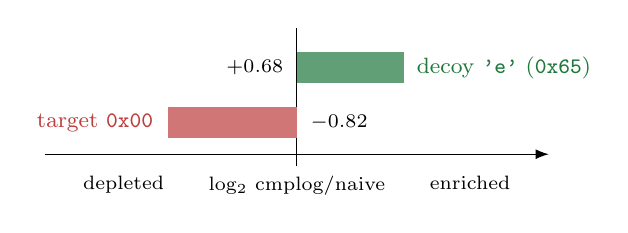
\begin{tikzpicture}[font=\footnotesize,>=Latex]
\draw[->] (-3.2,0) -- (3.2,0); \draw (0,-0.15)--(0,1.6);
\node[below] at (0,-0.15) {\scriptsize log$_2$ cmplog/naive};
\node[below] at (-2.2,-0.15) {\scriptsize depleted}; \node[below] at (2.2,-0.15) {\scriptsize enriched};
% target depleted
\fill[losc!70] (-1.64,0.2) rectangle (0,0.6);
\node[left,losc] at (-1.7,0.4) {target \texttt{0x00}};
\node[right] at (0.05,0.4) {\scriptsize $-0.82$};
% decoy enriched
\fill[winc!70] (0,0.9) rectangle (1.36,1.3);
\node[right,winc] at (1.4,1.1) {decoy \texttt{'e'} (\texttt{0x65})};
\node[left] at (-0.05,1.1) {\scriptsize $+0.68$};
\end{tikzpicture}\\[-1pt]
{\footnotesize I2S steers the cmplog corpus toward the wrong (decoy) operand and away from the value the branch needs.}
\end{center}

% =====================================================================
\section*{2.\ \ Blind substitution clobbers assembled structure \hfill {\normalsize\texttt{i2s\_anti\_structural\_byte\_corruption} ($n=10$)}}
Here there is \emph{no} rival operand. \emph{naive} havoc \emph{assembles} the
correct structural bytes, and \texttt{I2SRandReplace} blindly overwrites that exact
position with a logged value --- pure destruction, not redirection. The clean
fingerprint is shape \texttt{LWWW}: cmplog is the \emph{sole} loser (naive,
value\_profile, and vpc all resolve).

\begin{lstlisting}[style=c]
// harfbuzz  hb-ot-shaper-indic.cc
//   : initial_reordering_consonant_syllable()
if (start + 3 <= end &&   // <-- blocker (harfbuzz/5831): syllable >= 3 glyphs
    ...)                  //     needs a long repeated glyph run
\end{lstlisting}

\noindent The gate needs a Kannada syllable spanning $\ge 3$ glyphs, which naive
builds from long repeated multi-byte glyph runs. I2S overwrites bytes inside those
runs with harvested constants, shortening the run below the threshold, so the
cmplog corpus is depleted of the assembled structure.

\metricbox{operand\_enrichment}
{\texttt{signed\_target\_enrich}; the decoy fractions are small and \emph{diffuse} (no single dominant rival)}
{signed\_target\_enrich < -0.3}
{harfbuzz/5831 (\texttt{initial\_reordering\_consonant\_syllable:479}) --- the structural byte is present in 36\% of naive seeds but only 20\% of cmplog's; \texttt{signed\_target\_enrich}$=-13.6$ (saturated $=$ essentially erased at the operand offset), with only diffuse displacement (decoy fractions 3\% vs 0.8\%).}

\begin{center}
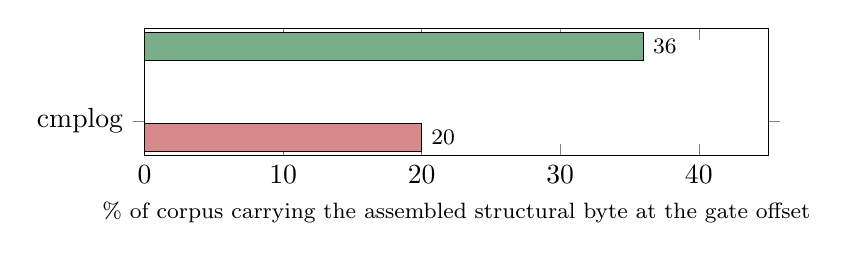
\begin{tikzpicture}
\begin{axis}[
  width=9.5cm, height=3.2cm, xbar, xmin=0, xmax=45,
  bar width=10pt, enlarge y limits=0.6,
  symbolic y coords={cmplog, naive},
  ytick=data, xtick={0,10,20,30,40},
  nodes near coords, every node near coord/.append style={font=\footnotesize},
  xlabel={\footnotesize \% of corpus carrying the assembled structural byte at the gate offset},
]
\addplot[fill=losc!60] coordinates {(20,cmplog)};
\addplot[fill=winc!60] coordinates {(36,naive)};
\end{axis}
\end{tikzpicture}\\[-1pt]
{\footnotesize naive assembles the structural byte; I2S overwrites it, so cmplog carries it far less often.}
\end{center}

% =====================================================================
\section*{3.\ \ A validity trap starves a semantic gate \hfill {\normalsize\texttt{i2s\_anti\_decoy\_overfit} ($n=14$)}}
The most subtle case. The decisive condition is \emph{semantic} --- not a byte at
an offset --- and I2S keeps re-asserting harvested \emph{structural} literals that
hold the input on a ``valid'' path, starving the branch of the semantic input it
needs.

\begin{lstlisting}[style=c]
// harfbuzz  hb-common.cc : hb_script_get_horizontal_direction()
switch (script) {
  ...
  case HB_SCRIPT_THAANA:     // <-- blocker (harfbuzz/5323)
    return HB_DIRECTION_RTL; //     needs Thaana-script text (U+0780..07BF)
}
\end{lstlisting}

\noindent The branch fires only when the decoded text is Thaana script. \emph{naive}
produces short, low-structure blobs that happen to decode to exotic scripts; but
I2S keeps splicing the harvested OpenType table tags \texttt{GPOS}/\texttt{GSUB}
into offsets 12--15, keeping the font structurally valid and ASCII/Latin --- so it
\emph{reaches} the \texttt{switch} every trial but never \emph{produces} the
script the gate wants.

\metricbox{operand\_enrichment}
{\texttt{signed\_target\_enrich} / \texttt{decoy\_enrich}. The byte decoy is a structural \emph{correlate} of the semantic gate, not the causal operand (a documented limit of a byte test on a semantic condition).}
{signed\_target\_enrich < -0.3}
{harfbuzz/5323 (\texttt{hb\_script\_get\_horizontal\_direction:594}, \texttt{case HB\_SCRIPT\_THAANA}) --- the \texttt{GPOS}/\texttt{GSUB} decoy fills 51\% of the cmplog corpus vs 0.05\% of naive's; \texttt{signed\_target\_enrich}$=-2.79$, \texttt{decoy\_enrich}$=+11.3$. The label still fires for the right reason: cmplog is depleted of what resolves the branch.}

\begin{center}
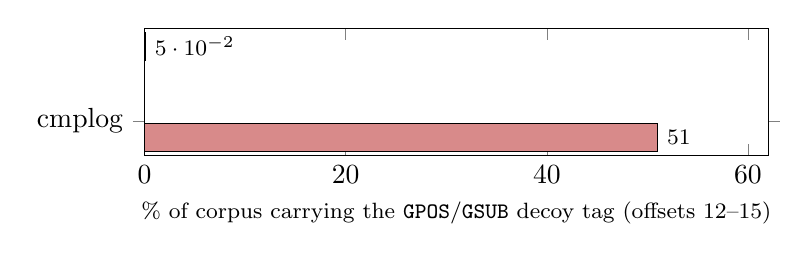
\begin{tikzpicture}
\begin{axis}[
  width=9.5cm, height=3.2cm, xbar, xmin=0, xmax=62,
  bar width=10pt, enlarge y limits=0.6,
  symbolic y coords={cmplog, naive},
  ytick=data, xtick={0,20,40,60},
  nodes near coords, every node near coord/.append style={font=\footnotesize},
  xlabel={\footnotesize \% of corpus carrying the \texttt{GPOS}/\texttt{GSUB} decoy tag (offsets 12--15)},
]
\addplot[fill=losc!60] coordinates {(51,cmplog)};
\addplot[fill=winc!60] coordinates {(0.05,naive)};
\end{axis}
\end{tikzpicture}\\[-1pt]
{\footnotesize I2S floods the corpus with valid table tags, keeping the font Latin and starving the Thaana-script gate.}
\end{center}

% =====================================================================
\section*{At a glance}
\begin{center}\small
\begin{tabular}{@{}p{3.5cm}clp{4.6cm}@{}}
\toprule
\textbf{Category} & \textbf{$n$} & \textbf{Example} & \textbf{What the decoy is} \\
\midrule
target\_depletion & 25 & libpng/3977 & one abundant \emph{rival} operand (\texttt{'e'}) \\
structural\_byte\_corruption & 10 & harfbuzz/5831 & none --- diffuse destruction of assembled bytes \\
decoy\_overfit & 14 & harfbuzz/5323 & a structural \emph{correlate} of a semantic gate (\texttt{GPOS}/\texttt{GSUB}) \\
\midrule
\textbf{I2S-A total} & \textbf{49} & & all share \texttt{signed\_target\_enrich}$<-0.3$ \\
\bottomrule
\end{tabular}
\end{center}

\noindent\footnotesize All counts and metric values are from \texttt{bench/dataset.jsonl}
and the per-branch analysis cards; the verify rules are the deterministic arbiter rules
(no LLM in the decision). libpng/3977 is verified against local source; the harfbuzz gates
are from their analysis cards (their corpora live on the other server).
\end{document}
